%%%%%%%%%%%%%%%%%%%%%%%%%%%%%%%%%%%%%%%%%%%%%%%%%%%%%%%%%%%%%%%%%%
%%%%%%%%%%%%%%%%%%%%%%%%%%%%%%%%%%%%%%%%%%%%%%%%%%%%%%%%%%%%%%%%%%
%%%%%%%%%%%%%%%%%%%%%%%%%%%%%%%%%%%%%%%%%%%%%%%%%%%%%%%%%%%%%%%%%%
\documentclass[prc, reprint, amsmath, floatfix,10pt]{revtex4-1}
%%%%%%%%%%%%%%%%%%%%%%%%%%%%%%%%%%%%%%%%%%%%%%%%%%%%%%%%%%%%%%%%%%
%%%%%%%%%%%%%%%%%%%%%%%%%%%%%%%%%%%%%%%%%%%%%%%%%%%%%%%%%%%%%%%%%%
%%%%%%%%%%%%%%%%%%%%%%%%%%%%%%%%%%%%%%%%%%%%%%%%%%%%%%%%%%%%%%%%%%

%
% Packages
%
\usepackage[utf8]{inputenc}
\usepackage[T1]{fontenc}
\usepackage{lipsum}
\usepackage{graphicx}
%\usepackage[np]{numprint}
\usepackage{amsmath}
\usepackage{amsfonts}
\usepackage{amssymb}
\usepackage{calrsfs}
\usepackage[left=2cm,right=2cm,top=2cm,bottom=2cm]{geometry}
\usepackage[mathscr]{euscript}
\usepackage{multirow}
%\usepackage{longtable}

% Gráficos em Tikz, terão que ser convertidos antes de submeter
\usepackage{tikz}
\usepackage{gnuplot-lua-tikz}

%
% Macros
%
\newcommand{\tr}{\rm{Tr}}
\newcommand{\mean}[1]{\left\langle{#1}\right\rangle}
\newcommand{\comment}[1]{{\bf\textit{#1}}}

%%%%%%%%%%%%%%%%
%%%%%%%%%%%%%%%%
\begin{document}
%%%%%%%%%%%%%%%%
%%%%%%%%%%%%%%%%

%
%%
%%%
%%%% Front Matter
%%%
%%
%

\title{Hadron-quark phase transition and possible conversion of a metastable star to a quark star}

\author{Clebson A. Graeff}
\affiliation{Universidade Tecnológica Federal do Paraná, campus Pato Branco \\ Via do Conhecimento, Km 1 CEP 85503-390 Pato Branco -- PR, Brazil}
\email{cgraeff@utfpr.edu.br}

\author{Marcelo D. Alloy}
\affiliation{Departamento de Ciências Exatas e Educação, Universidade Federal de Santa Catarina, Blumenau, SC, CEP 89.065-300, Brazil}
\email{marcelo.alloy@ufsc.br}

\author{Constança Providência}
\affiliation{Departamento de Física, Universidade de Coimbra, 3004-516 Coimbra, Portugal}
\email{cp@teor.fis.uc.pt}

\author{Débora P. Menezes}
\affiliation{Departamento de Física, Universidade Federal de Santa Catarina, Florianópolis, SC, CP 476, CEP 88.040-900, Brazil}
\email{debora.p.m@ufsc.br}

%%%

\begin{abstract}
An article usually includes an abstract, a concise summary of the work
covered at length in the main body of the article. 
\begin{description}
\item[Usage]
Secondary publications and information retrieval purposes.
\item[PACS numbers]
May be entered using the \verb+\pacs{#1}+ command.
\item[Structure]
You may use the \texttt{description} environment to structure your abstract;
use the optional argument of the \verb+\item+ command to give the category of each item. 
\end{description}
\end{abstract}

%%%

\pacs{Valid PACS appear here}

%%%

\maketitle

%
%%
%%%
%%%% Main Matter
%%%
%%
%

%%%%%%%%%%%%%%%%%%%%%%
\section{Introduction}
%%%%%%%%%%%%%%%%%%%%%%

The complete understanding of the QCD phase diagram represents a challenge in both theoretical and experimental physics. While many of the features it aims to describe can be tested in earth experiments, other aspects related to matter under extreme conditions, can only be infered from lattice QCD (LQCD) \cite{lqcd} or from observational results of astrophysical objects.

From the experimental point of view, the Beam Energy Scan (BES-I, BES-II) programs at RHIC have been given data on signatures of a first order phase transition and
the possible existence and location of the critical end point (CEP) \cite{BES}, which would indicate the end of the first order phase transition and the beginning of a different kind of transition. Future experiments to take place at the FAIR facility at GSI \cite{FAIR} , NICA at the JINR \cite{NICA} and the NA61/SHINE program at SPS (CERN)  \cite{NA61} will also contribute to these still unknwon aspects.

From the LQCD site, the transition is believed to be a cross over, reforcing the idea of the existence of a critical end point. However, due to some numerical difficulties as the {\it sign problem} and the need of expensive computational facilities, the whole diagram is not expected to be covered in a near future.

The improvement of the observational results of compact objects are also expected soon from the future x-ray telescopes, such as NICER \cite{NICER} and Athena \cite{ATHENA}, contributing to the understanding of the low temperature-high density region of the phase diagram.

Meanwhile, effective models remain a good source of qualitative results and the present work helps in advancing with our knowledge. It is worth mentioning that at low temperatures the phase transition can take place at two steps by first restoring the chiral transition where matter is still confined giving rise to a phase known as quarkyonic \cite{quarkyonic}, and only later on, suffering the transition to the deconfined phase. 

We focus our work on two major points: the investigation of the phase transition from hadronic matter to quark matter at zero temperature and the possibility that this transtion is correlated with a conversion from a mestastable hadronic to a stable quark star.

Considerations on the phase transition at zero temperature have already been done in many works \cite{Cavagnoli2011, Tsue2010, Lee2013}, but we do believe the formalism we present next is more adequate. If the appearance of a quarkyonic phase is taken seriously, the model to be used should consider chiral symmetry in both hadronic and quark phases. In \cite{Cavagnoli2011}, the phase transition was investigated with the help of two different models, namely, the non-linear Walecka model (NLWM) for the hadronic phase and the MIT bag model for the quark phase. A formalism more similar with what we have in mind was used at zero \cite{Tsue2010} and finite \cite{Lee2013} temperature, where the Nambu-Jona-Lasinio type models were used for both phases.

In \cite{Cavagnoli2011} the authors study the phase transition from hadrons to a quark-gluon plasma in asymmetric matter using a two phase model in which the hadron phase is described by the non-linear Walecka Model (NLWM), while the quark phase is described by the MIT Bag Model, analysing the features that depend on the isospin and may be relevant in a phenomenological description of heavy-ion collision. \comment{(Ipsis litteris)}

The phase transition is also considered at zero~\cite{Tsue2010} and finite~\cite{Lee2013} temperatures, but using Nambu--Jona-Lasinio type models for both phases. Again, a simple two phase model is employed. To describe the hadron phase, the standard NJL model with vector interaction is extended to include a scalar-vector channel, which renders the model capable of saturation at low densities.

We revisit the approach of~\cite{Tsue2010} and~\cite{Lee2013} whilst using a further extended model~\cite{Pais2016} which uses additional channels to achieve a better description of the symmetry energy. \comment{(Importância disso aqui.)} Albeit the authors also refer to this extension as eNJL, here we will name this new extension PPM to avoid confusion.

The effects of the different channels are: the term in $G_v$ simulates a chiral-invariant short-range repulsion between the nucleons, the term in $G_{sv}$ accounts for the density dependence of the scalar coupling, the term in $G_\rho$ allows the description of isospin asymmetric matter, and the terms in $G_{\omega\rho}$ and $G_{s\rho}$ make the symmetry energy softer. For nuclear matter, the NJL model leads to binding, but the binding energy per particle does not have a mininum except at a rather high density where the nucleon mass is small or vanishing. The introduction of the term in $G_{sv}$ corrects this.\comment{(Quase ipsis litteris de \cite{Pais2016}).}


\comment{(Quando estiver finalizado, adicionar descrição da organização aqui.)}

%%%%%%%%%%%%%%%%%%%
\section{Formalism}
%%%%%%%%%%%%%%%%%%%

%%%%%%%%%%%%%%%%%%%%%%%%%%%%%%%%%%%%%
\subsection{Quark Matter - NJL SU(2)}\label{NJLSU2}
%%%%%%%%%%%%%%%%%%%%%%%%%%%%%%%%%%%%%


The quark phase is described by a SU(2) NJL model lagrangian, including a vector term, given by \cite{Buballa2005}
\begin{equation}\label{Eq:LagNJL-SU2-Bub}
\begin{split}
	\mathscr{L} =&~ \bar{\psi}(i\gamma^\mu\partial_\mu - m_0)\psi \\
	&+ G_s[(\bar{\psi}\psi)^2 + (\bar{\psi}i\gamma_5\vec{\tau}\psi)^2] - G_v(\bar{\psi}\gamma^\mu \psi)^2.
\end{split}
\end{equation}
%
Here $\psi$ represents the quark field, $m_0$ the quark bare mass, and $G_s$ and $G_v$ are coupling constants that are chosen by fitting the pion mass $m_\pi = 135.0~\rm{MeV}$ and its decay constant $f_\pi = 92.4~\rm{MeV}$. As the theory is non-renormalizable, a momentum cutoff $\Lambda$ is employed, which acts as a new parameter.

From the lagrangian $\mathscr{L}$, the hamiltonian density $\mathscr{H}$ can be obtained, which leads to the thermodynamic potential per volume $V$ at temperature $T$ by means of
\begin{equation}
	\omega(T, \mu) = -\frac{T}{V} \ln \tr \exp\left(-\frac{1}{T}\int d^3x(\mathscr{H} - \mu\psi^\dagger\psi\right),
\end{equation}
%
where $\tr$ stands for a trace over all states of the system, resulting in \cite{Buballa1996}
\begin{equation}\label{Eq:Pot_Termo_Temp_zero}
\begin{split}
	\omega(\mu; m, \mu_R) =&~ \omega_m^{(\rm{vac})} + \omega_m^{(\rm{med})}(\mu_R) \\
	&+ \frac{(m - m_0)^2}{4G_s} - \frac{(\mu - \mu_R)^2}{4G_v} +  \textrm{const.},
\end{split}
\end{equation}
%
with
\begin{align}
	\omega_m^{(\rm{vac})} &= -(2 n_f n_c) \int \frac{d^3p}{(2\pi)^3} E_p\\
	\omega_m^{(\rm{med})}(\mu_R) &= - (2n_f n_c) \int\frac{d^3p}{(2 \pi)^3} (\mu_R - E_p) \theta(p_F -p),
\end{align}
%
at the zero temperature limit in the mean-field approximation. Here $n_f$ and $n_c$ stand for the number of flavors and the number of colors, respectively, and $E_p = \sqrt{p^2 + m^2}$. The Fermi momentum of the quarks is represented by $p_F$ and $\theta(p_F - p)$ stands for the step function.

The renormalized chemical potential $\mu_R$ and the constituent mass $m$ are obtained by requiring that $\partial \omega / \partial \mu_R = 0$ and $\partial \omega / \partial m = 0$, respectively, resulting in
\begin{align}
	\mu_R &= \mu - 2 G_v \rho \\
	m &= m_0 - 2 G_s \rho_s
\end{align}
%
with
\begin{align}
	\rho &= n_c \rho_B = \frac{n_f n_c}{3\pi^2} p_F^3 \\
	\rho_s &= \langle \bar\psi\psi\rangle = - 2 n_f n_c \int\frac{d^3p}{(2\pi)^3} \frac{m}{E_p}(1 - \theta(p_F - p)) \\
	\mu_R &= \sqrt{p_F^2 + m^2},
\end{align}
%
where $\rho_B$ stands for the barionic density.

The constant in the potential has no physical meaning, consequently, it may be chosen so that at $T = \mu = 0$ the thermodynamic potential is zero at the value $m = m_{\rm{vac}}$ which minimizes $\omega$. This process may be represented by 
\begin{equation}
	\tilde\omega(\mu; m, \mu_R) = \omega(\mu; m, \mu_R) - \omega(0, 0; m_{\rm{vac}}, 0),
\end{equation}
%
so that the quantities we are interested in --~the pressure $P$ and the energy density $\varepsilon$~-- are obtained through
\begin{align}
		P &= -\tilde\omega(\mu; m, \mu_R) \label{Exp_pressao_T}\\
		\varepsilon &= -p + \mu \rho. \label{Exp_energia_T}
\end{align}
	
The equations are solved self-consistently for each value of $\rho$ or $\mu$ (in this case $p_F = \sqrt{\mu_R^2 - m^2}\theta(\mu_R^2 - m^2)$).

\begin{table}[!htpb]
\centering
\caption{Parameters sets for the lagrangian density~\eqref{Eq:LagNJL-SU2-Bub} \cite{Buballa1996, Buballa2005}. \label{Tab:Parametros_NJL}}
\begin{ruledtabular}
\begin{tabular}{lccccc}
Model &  $\Lambda$ & $G_s$ ($\rm{fm}^2$) & $G_v$ ($\rm{fm}^2$) & $m_0$ (MeV) & $m$ (MeV) \\
\hline
Buballa-1 & 650 & 0.19721 & -- & 0 & 313 \\
Buballa-2 & 600 & 0.26498 & -- & 0 & 400 \\
Buballa-3 & 570 & 0.34034 & -- & 0 & 500 \\
%BuballaR-1 & 664.3 & 0.18176 & $\propto G_s$ & 5.0 & 300 \\
BuballaR-2 & 587.9 & 0.27449 & $\propto G_s$ & 5.6 & 400 \\
%BuballaR-3 & 569.3 & 0.33759 & $\propto G_s$ & 5.5 & 500 \\
%BuballaR-4 & 568.6 & 0.38178 & $\propto G_s$ & 5.1 & 600
\end{tabular}
\end{ruledtabular}
\end{table}

%%%%%%%%%%%%%%%%%%%%%%%%%%%%%%%%%%%%%
\subsection{Quark Matter - NJL SU(3)}\label{NJLSU3}
%%%%%%%%%%%%%%%%%%%%%%%%%%%%%%%%%%%%%

The another way to describe dense matter in a quark phase is from the
SU(3) version of Nambu Jona Lasinio model with repulsive vector interaction. In this case,
the Lagrangian density is given by
\begin{equation}
\mathscr{L}=\overline{\psi}[\gamma_\mu(i\partial^\mu)-\widehat{m}_f]\psi+
\mathscr{L}_{sym}+\mathscr{L}_{det}+\mathscr{L}_{vec},
\end{equation}
where $\mathscr{L}_{sym}$, $\mathscr{L}_{det}$ and $\mathscr{L}_{vec}$ are given by
\begin{eqnarray}
\mathscr{L}_{sym}&=&G_s\sum_{a=0}^8[(\overline{\psi}\lambda_a\psi)^2+(\overline{\psi}i\gamma_5\lambda_a\psi)^2],\nonumber\\
\mathscr{L}_{det}&=&-K\{\mbox{det}[\overline{\psi}(1+\gamma_5)\psi]+\mbox{det}[\overline{\psi}(1-\gamma_5)\psi]\},\nonumber\\
%\mathscr{L}_{vec}&=&-G_s\sum_{a=0}^8[(\overline{\psi}\gamma_\mu\lambda_a\psi)^2+(\overline{\psi}\gamma_5\gamma_\mu\lambda_a\psi)^2],
\mathscr{L}_{vec}&=&-G_s(\overline{\psi}\gamma^\mu\psi)^2,\nonumber
\end{eqnarray}
where $\psi(u,d,s)$ represents a quark field with three flavors,
$\widehat{m}_f=\mbox{diag}(m_u,m_d,m_s)$ is the quark current mass,
$\lambda_0=\sqrt{2/3}I$ where $I$ is the unit matrix in three flavor space,
$\lambda_a(0\leq a \leq 8)$ are the U(3) flavor matrices. 
To obtain effective quark masses $M_i$ we must minimizing thermodynamical potential 
given by $\omega=-P=\varepsilon-\sum_{i=u,d,s}\mu_i\rho_i$, where $\varepsilon$ is the energy
density given by
\begin{eqnarray}
\varepsilon&=&-2N_c\sum_{i=u,d,s}\int\frac{d^3p}{(2\pi)^3}\frac{p^2+m_iM_i}{E_i}\theta(\Lambda^2-p_{Fi}^2)\nonumber\\
&-&2G_s\sum_{i=u,d,s}\langle\overline{q}_iq_i\rangle^2-2K\langle\overline{u}u\rangle\langle\overline{d}d\rangle\langle\overline{s}s\rangle\\
&+&2G_v\rho^2,\nonumber
\end{eqnarray}
where $N_c=3$, $E_i=\sqrt{p_i^2+M_i^2}$, $p_{Fi}=\sqrt{\widetilde{\mu}_i^2-M_i^2}$ and $\rho=\rho_u+\rho_d+\rho_s$.
The renormalized chemical potential $\widetilde{\mu}_i$ is given by
\begin{equation}
\widetilde{\mu}_i=\mu_i-2G_v\rho_i,
\end{equation}
where $i$ refers to the flavor and $\rho_i$ refers to the respective quark number densities. Thus,
minimizing $\omega$, we obtain in mean-field approach the following gap equations
\begin{equation}
M_i=m_i-4G_s\phi_i+2K\phi_j\phi_k,
\end{equation}
with $(i,j,k)$ being any permutation of $(u,d,s)$ and $\phi_i$ 
stands for the scalar condensate of the $i$-flavor quark.
The parameters set used to evaluate equation of state for the NJL SU(3) model are
$\Lambda=631.4$ MeV, $G_s\Lambda^2=1.835$, $K\Lambda^5=9.29$, $m_{u,d}=5.5$ MeV, $m_s=135.7$ MeV
and $G_v=xG_s$, where $x$ is a free parameter which we vary such that $0<x<1$, according in Ref. \cite{PhysRevD.64.043005} 

%%%%%%%%%%%%%%%%%%%%%%%%%%
\subsection{Hadron Matter}\label{NJLHM}
%%%%%%%%%%%%%%%%%%%%%%%%%%

Even though the original NJL model is unable to describe the saturation properties of the nuclear matter, this can be fixed by an extended version which include a scalar-vector channel (eNJL)~\cite{Koch1987}. Other channels that can help the description of other properties as discussed in the Introduction are also included in this ... The lagrangian density of the PPM model is given by~\cite{Pais2016}
\begin{equation}\label{Eq:Lagrangiana_eNLJ_Pais}
\begin{split}
	\mathscr{L} =&~ \bar{\psi}(i\gamma^\mu\partial_\mu - m_0)\psi \\
	& + G_s[(\bar{\psi}\psi)^2 + (\bar{\psi}i\gamma_5\vec{\tau}\psi)^2] \\
	& - G_v(\bar{\psi}\gamma^\mu\psi)^2 - G_{sv}[(\bar{\psi}\psi)^2 + (\bar{\psi}i\gamma_5\vec{\tau}\psi)^2](\bar{\psi}\gamma^\mu\psi)^2 \\
	& - G_\rho[(\bar{\psi}\gamma^\mu\vec{\tau}\psi)^2 + (\bar{\psi}\gamma_5\gamma^\mu\vec{\tau}\psi)^2] \\
	& - G_{v\rho}(\bar{\psi}\gamma^\mu\psi)^2[(\bar{\psi}\gamma^\mu\vec{\tau}\psi)^2 + (\bar{\psi}\gamma_5\gamma^\mu\vec{\tau}\psi)^2] \\
	& - G_{s\rho} [(\bar{\psi}\psi)^2 + (\bar{\psi}i\gamma_5\vec{\tau}\psi)^2][(\bar{\psi}\gamma^\mu\vec{\tau}\psi)^2 + (\bar{\psi}\gamma_5\gamma^\mu\vec{\tau}\psi)^2],
\end{split}
\end{equation}
%
where $\psi$ represents the nucleon field and the constants $G_i$ represents the coupling constants for the different channels. As in the quark case, the theory is renormalized via a three momentum cutoff $\Lambda$.

The thermodynamic potential is obtained from~\eqref{Eq:Lagrangiana_eNLJ_Pais} in the same way as for the quark case and is given by
\begin{equation}\label{Eq:potencial_termodinamico}
\begin{split}
	\omega(\mu) =&~ \varepsilon_{\rm{kin}} + m\rho_s - G_s\rho_s^2 + G_v\rho_B^2 + G_{sv}\rho_s^2\rho_B^2 + G_\rho\rho_3^2 \\
	&+ G_{v\rho}\rho_B^2\rho_3^2 + G_{s\rho}\rho_s^2\rho_3^2 - \mu_p\rho_B^p - \mu_n\rho_B^n,
\end{split}
\end{equation}
%
where $\rho_B$ is the total barionic density, which is the sum of the proton $\rho_B^p$ and neutron $\rho_B^n$ barionic densities, while $\rho_3 = \rho_B^p - \rho_B^n$. At zero temperature, those densities are given by
\begin{equation}
	\rho_B^i = \int_0^{p_F^i}\frac{dp}{\pi^2}p^2; \qquad i = p,n
\end{equation}
%
where $p_F^i$ stands for the Fermi momentum of each particle. The kinectic energy contribution is given by
\begin{equation}
	\varepsilon_{\rm{kin}} = 2 n_c \sum_i \int \frac{d^3p}{(2\pi)^3}\frac{p^2}{E_p^i}(1 - \theta(p_F^i - p))\theta(\Lambda^2 - p^2).
\end{equation}

The effective mass $m$ and the chemical potentials appearing in the thermodynamic potencial $\omega$ are determined by requiring that $\partial\omega/\partial m = 0$ and $\partial\omega/\partial p_F^i = $, resulting in
\begin{align}\label{Eq:Gap}
	m &= m_0 - 2G_s\rho_s + 2G_{sv}\rho_s\rho^2 + 2 G_{s\rho}\rho_s\rho_3^2 \\
	\mu_i &= E_{p_F}^i + 2G_v\rho + 2G_{sv}\rho\rho_s^2 \pm 2G_\rho\rho_3+2G_{v\rho}\rho_3^2\rho \nonumber \\
	&\phantom{=} \pm 2G_{v\rho}\rho^2\rho_3 \pm 2 G_{s\rho}\rho_3\rho_s^2,
\end{align}
%
with $i = p,n$, and e $E_{p_F}^i = \sqrt{M^2 + (p_F^i)^2}$. The scalar density $\rho_s$ is given by sum of the proton and neutron scalar densities
\begin{equation}
	\rho_s^i = - 2 n_c \int \frac{d^3p}{(2\pi)^3}\frac{m_0^i m_i}{E_p^i}\theta(p_F - p)\theta(\Lambda^2 - p^2)
\end{equation}
%
where $i = p, n$.

The equations of state can be obtained from
\begin{align}
	P &= -\omega(\mu) + \omega_{\rm{vac}} \\
	\varepsilon &= -P + \mu_p \rho_B^p + \mu_n \rho_B^n,
\end{align}
%
where $\omega_{\rm{vac}} = \omega(T = 0, \mu = 0, m = m_N)$, with $m_N$ representing the nucleon mass. 

\begin{table*}
\caption{Conjuntos de parâmetros para a lagrangiana~\eqref{Eq:Lagrangiana_eNLJ_Pais}\cite{Pais2016}. \label{Tab:Parametros_eNJL}}
\begin{ruledtabular}
\begin{tabular}{lcccccccc}
Model & $G_s$ ($\rm{fm}^2$) & $G_v$ ($\rm{fm}^2$) & $G_{sv}$ ($\rm{fm}^8$) & $G_\rho$ ($\rm{fm}^2$) & $G_{v\rho}$ ($\rm{fm}^8$) & $G_{s\rho}$ ($\rm{fm}^8$) & $\Lambda$ (MeV) & $m$ (MeV) \\
\hline
eNJL1 & 4.855 & 4.65 & -6.583 & 0.5876 & 0 & 0 & 388.189 & 0 \\
eNJL1$\omega\rho$1 & 4.855 & 4.65 & -6.583 & 0.5976 & -1 & 0 & 388.189 & 0 \\
eNJL1$\omega\rho$2 & 4.855 & 4.65 & -6.583 & 0.6476 & -6 & 0 & 388.189 & 0 \\
eNJL2 & 3.8 & 3.8 & -4.228 & 0.6313 & 0 & 0 & 422.384 & 0 \\
eNJL2$\omega\rho$1 & 3.8 & 3.8 & -4.228 & 0.6413 & -1 & 0 & 422.384 & 0 \\
eNJL3 & 1.93 & 3.0 & -1.8 & 0.65 & 0 & 0 & 534.815 & 0 \\
eNJL3$\sigma\rho$1 & 1.93 & 3.0 & -1.8 & 0.0269 & 0 & 0.5 & 534.815 & 0 \\
eNJL1m & 1.3833 & 1.781 & -2.943 & 0.7 & 0 & 0 & 478.248 & 450 \\
eNJL1m$\sigma\rho$1 & 1.3833 & 1.781 & -2.943 & 0.0739 & 0 & 1 & 478.248 & 450 \\
eNJL2m & 1.078 & 1.955 & -2.74 & 0.75 & 0 & 0 & 502.466 & 450 \\
eNJL2m$\sigma\rho$1 & 1.078 & 1.955 & -2.74 & -0.1114 & 0 & 1 & 502.466 & 450 \\
\end{tabular}
\end{ruledtabular}
\end{table*}

%%%%%%%%%%%%%%%%%%
\section{Binodals}
%%%%%%%%%%%%%%%%%%

The QCD phase-diagram is characterized by potentially multiple phases, whose phase separation boundaries are referred as \emph{binodals} \cite{Mueller1995}. Over those boundaries, the phases from the regions of either side of the boundary can coexist. The binodals may be determined using the Gibbs' conditions \cite{Cavagnoli2011}:
\begin{align}
\mu_B^Q &= \mu_B^H \\
T^Q &= T^H \\
P^Q &= P^H
\end{align}
%
where the indexes $H$ and $Q$ refer to the hadrons and quarks phases. The chemical potentials are given by
\begin{align}
	\mu_B^H &= \frac{\mu_p + \mu_n}{2} \\
	\mu_B^Q &= \frac{3}{2} (\mu_u + \mu_d) = 3 \mu_q.
\end{align}
%
The phase coexistence may be obtained simply by plotting $P^i \times \mu_B^i$, $i = Q, H$, and looking for the intersection of both lines (see Fig.~\ref{Fig:Intersection}). The absence of intersections imply that there are no phase transitions in the range shown (see Fig.~\ref{Fig:NoIntersection}).

\begin{figure}
	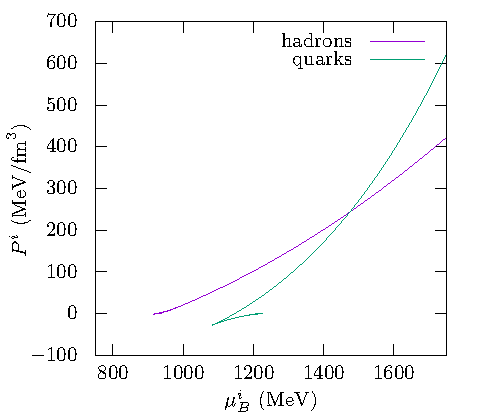
\includegraphics[width=\linewidth]{graph/BuballaR_2-eNJL1OmegaRho1-quark-hadron_phase_transition.pdf}
	\caption{Example of a combination of parameters sets for which there is a phase transition. Quarks: BuballaR-2; Hadrons: eNJL1$\omega\rho$1. \label{Fig:Intersection}}
\end{figure}

\begin{figure}
	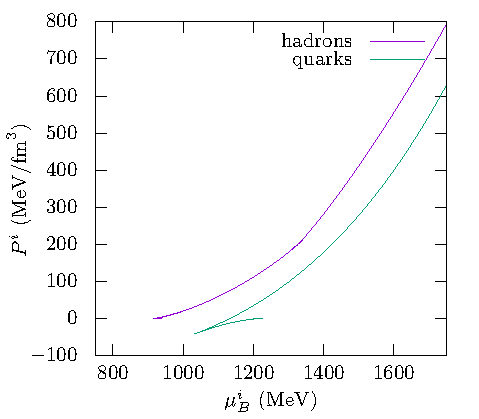
\includegraphics[width=\linewidth]{graph/Buballa_2-eNJL1m-quark-hadron_phase_transition.pdf}
	\caption{Example of a combination of parameters sets for which no phase transition happens. Quarks: Buballa-2; Hadrons: eNJL1m. \label{Fig:NoIntersection}}
\end{figure}

\begin{figure}
	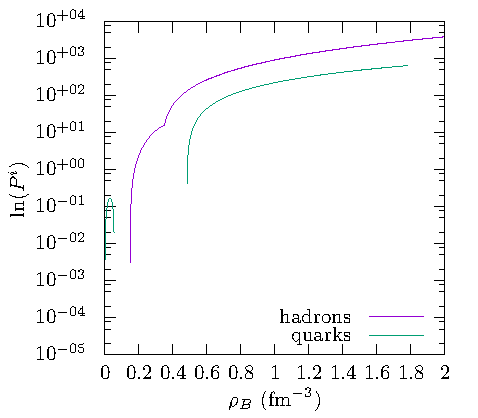
\includegraphics[width=\linewidth]{graph/BuballaR_2-eNJL1OmegaRho1-quark-hadron_phase_transition2.pdf}
	\caption{\comment{O que as descontinuidades significam?} Quarks: BuballaR-2; Hadrons: eNJL1$\omega\rho$1.}
\end{figure}

We determine the value of chemical potential $\mu_B^i$ for which the phase transition takes place for combinations of the parameters sets from Tables~\ref{Tab:Parametros_NJL} e~\ref{Tab:Parametros_eNJL}. Furthermore, we restrict our treatment of the hadron phase to symmetric matter due to the fact that in our treatment of the quark phase the proportion of $u$ and $d$ quarks is always 50\% of each particle. This reflects the fact that both particles are assumed to have the same bare mass and the same chemical potential.

The results so obtained are displayed in Table~\ref{Tab:Transition_chemical_pot}. In particular we may note that no combination involving the BuballaR-2 set with $G_V \neq 0$ present a transition.


\begin{table}[!htpb]
\centering
\caption{Chemical potential $\mu_B^i$ at crossing point por different parameterization combinations. For BuballaR-2 in this table we have $G_V = 0$.\label{Tab:Transition_chemical_pot}}
\begin{ruledtabular}
\begin{tabular}{cccc}
Quarks & Hadrons & $\mu_B^i$ (MeV) & $P^i$ (MeV/fm$^3$) \\
\hline
Buballa-1 & eNJL1 & 1244 & 122\\
Buballa-1 & eNJL1$\omega\rho$1 & 1244 & 122 \\
Buballa-1 & eNJL1$\omega\rho$2 & 1244 & 122 \\
Buballa-1 & eNJL2 & 1373 & 216\\
Buballa-1 & eNJL2m & 1279 & 145\\
Buballa-1 & eNJL2m$\sigma\rho$1 & 1279 & 145 \\
Buballa-1 & eNJL2$\omega\rho$1 & 1373 & 216 \\
Buballa-1 & eNJL3 & 1313 & 169\\
Buballa-1 & eNJL3$\sigma\rho$1 & 1313 & 169 \\
Buballa-2 & eNJL1 & 1460 & 235\\
Buballa-2 & eNJL1$\omega\rho$1 & 1460 & 235 \\
Buballa-2 & eNJL1$\omega\rho$2 & 1460 & 235 \\
Buballa-2 & eNJL2 & 1557 & 343\\
Buballa-2 & eNJL2m & 1675 & 506\\
Buballa-2 & eNJL2m$\sigma\rho$1 & 1675 & 506 \\
Buballa-2 & eNJL2$\omega\rho$1 & 1557 & 343 \\
Buballa-2 & eNJL3 & 1571 & 361 \\
Buballa-2 & eNJL3$\sigma\rho$1 & 1571 & 361 \\
Buballa-3 & eNJL1 & 1615 & 330\\
Buballa-3 & eNJL1$\omega\rho$1 & 1615 & 331 \\
Buballa-3 & eNJL1$\omega\rho$2 & 1615 & 331 \\
Buballa-3 & eNJL2 & 1700 & 456 \\
Buballa-3 & eNJL2$\omega\rho$1 & 1700 & 456 \\
Buballa-3 & eNJL3 & 1744 & 530\\
Buballa-3 & eNJL3$\sigma\rho$1 & 1744 & 530 \\
BuballaR-2 & eNJL1 & 1475 & 244 \\
BuballaR-2 & eNJL1$\omega\rho$1 & 1475 & 244 \\
BuballaR-2 & eNJL1$\omega\rho$2 & 1475 & 244 \\
BuballaR-2 & eNJL2 & 1570 & 354 \\
BuballaR-2 & eNJL2m & 1730 & 587\\
BuballaR-2 & eNJL2m$\sigma\rho$1 & 1730 & 587 \\
BuballaR-2 & eNJL2$\omega\rho$1 & 1570 & 354 \\
BuballaR-2 & eNJL3 & 1587 & 376 \\
BuballaR-2 & eNJL3$\sigma\rho$1 & 1587 & 376 \\
\end{tabular}
\end{ruledtabular}
\end{table}


\section{Metastable stars}
The equations of state obtained in a previous sections can not be used to describe
stellar matter because electric charge neutrality and $\beta$-equilibrium are not take
account. To turn them appropriate to describe stellar matter we must introduce leptons in
the system by adding in Lagrangian density of each model the Lagrangian density that
describe the behavior of the free gas of leptons given by
\begin{equation}
\mathscr{L}=\overline{\psi}_l[\gamma_\mu(i\partial^\mu -m_l]\psi_l,
\end{equation}
where $l$ refers to the leptons, and impose the following constraints on chemical
potential and number density
\begin{eqnarray}
\mu_s=\mu_d=\mu_u+\mu_e, \qquad \mu_e=\mu_u, \\
\rho_e+\rho_u=\frac{1}{3}(2\rho_u-\rho_d-\rho_s).
\end{eqnarray}
For the lepton densities we have
\begin{equation}
\rho_l=g_l\int_0^{k_{Fl}}\frac{d^3p}{(2\pi)^3},
\end{equation}
where $k_{Fl}=\sqrt{\mu_l^2-m_l^2}$ and $g_l$ is  2 for charged leptons e 1 for neutrinos.
By adding leptons in the system,
the pressure and energy density will increase by $\varepsilon_l$ and $P_l$ given by
\begin{eqnarray}
\varepsilon_l&=&\frac{1}{2\pi^2}\sum_lg_l\int_0^{k_{Fl}} dp\sqrt{p^2+m_l^2},\\
P_l&=&\frac{1}{6\pi^2}\sum_lg_l\int_0^{k_{Fl}} \frac{p^4dp}{\sqrt{p^2+m_l^2}}.
\end{eqnarray}
Now we can turn our attention to construct a sequence of compact stars for each
equation of state obtained from the models described in the sections (\ref{NJLSU2}),
(\ref{NJLSU3}) and (\ref{NJLHM}) with $\beta-$equilibrium and electric charge neutrality.
The sequence of compact stars are obtained by using the equation of state, $\varepsilon=\varepsilon(P)$,
as input for the Tolman-Oppenheimer-Volkoff (TOV) equations given by
\begin{eqnarray}
\frac{dP}{dr}&=&-\frac{(\varepsilon+P)(M(r)+4\pi r^3P)}{r(r-2M(r))},\\
\frac{dM}{dr}&=&4\pi r^2\varepsilon,\\
\frac{dM_B}{dr}&=&\frac{4\pi r^2\rho_B}{1-2M(r)/r},
\end{eqnarray}
where $r$ is a radial coordinate of the compact star, $P$ and $\varepsilon$ are the
pressure and energy density, $M(r)$ and $M_B(r)$ are the gravitational mass and barionic
mass enclosed in a sphere of radius r and $\rho_B$ is the barionic density. To solve TOV
equations we need to impose boundary conditions given by $P(R)=0$ and $P(0)=P_c$,
where $R$ is the star radius and $P_c$ is the central pressure. 
Thus, $M(R)$ and $M_B(R)$ are total gravitational mass and total barionic
mass of the compact star. Sequence of compact stars means that for each equation of state we have 
a set of solutions of TOV equation, where each solution is one possible star of gravitational
mass $M$, barionic mass $M_B$, radius $R$ and central pressure $P_c$.

A compact star consisting only of hadrons (NS), a compact star with no fraction of 
deconfined quark matter, and having a central pressure $P_c$ larger than the transition
pressure $P_0$ for the formation of quark phase matter is metastable 
\cite{2002NuPhS.113..268B, 2003ApJ...586.1250B, 2004ApJ...614..314B} to the
conversion to a quark star (QS). The conversion of a metastable hadron star to a
quark star is a process that release a huge amount of energy ($\sim 10^{53}$) erg, which could
be the energy source of gamma-ray burst. The table \ref{table:ns-qs} show some values of
released energy in the process of conversion of a metastable hadron star to a quark star.
We assume barionic mass constant in the conversion process.



\begin{table*}[!htpb]

\centering
\caption{Energy released $\Delta E$ in evolution of an metastable Neutron Star (NS) to Quark Stars (QS) assuming $M_B$ constant during evolution process.}\label{table:ns-qs}
\begin{ruledtabular}
\begin{tabular}{cccccc}
NS                    & $P_0$ (MeV/fm$^3$) & $P_c$ (MeV/fm$^3$) & QS                                 &  MB $(M_\odot)$ & $\Delta E$ (ergs)      \\ \hline
\multirow{6}{*}{eNJL1}&\multirow{6}{*}{122}& \multirow{3}{*}{38.03}  & x=0.7 & 1.44   & $3.36\times 10^{53}$ \\ \cline{4-6} 
                      & 				   &   						 & x=0.8 & 1.44   & $3.54\times 10^{53}$ \\ \cline{4-6} 
                      & 				   &  						 & x=0.9 & 1.44   & $3.64\times 10^{53}$ \\ \cline{3-6} 
                      & 				   & \multirow{3}{*}{100.83} & x=0.7 & 2.00   & $5.74\times 10^{53}$ \\ \cline{4-6} 
                      & 				   & 						 & x=0.8 & 2.00   & $6.01\times 10^{53}$ \\ \cline{4-6} 
                      &					   &  						 & x=0.9 & 2.00   & $6.11\times 10^{53}$ \\ \hline
\multirow{6}{*}{eNJL2}&\multirow{6}{*}{216}& \multirow{3}{*}{42.62}	 & x=0.7 & 1.44   & $3.37\times 10^{53}$ \\ \cline{4-6} 
                      & 				   & 						 & x=0.8 & 1.44   & $3.54\times 10^{53}$ \\ \cline{4-6} 
                      & 				   & 						 & x=0.9 & 1.44   & $3.65\times 10^{53}$ \\ \cline{3-6} 
                      & 				   & \multirow{3}{*}{146.15} & x=0.7 & 2.00   & $5.78\times 10^{53}$ \\ \cline{4-6} 
                      & 				   & 						 & x=0.8 & 2.00   & $6.06\times 10^{53}$ \\ \cline{4-6} 
                      & 				   & 				  	     & x=0.9 & 2.00   & $6.16\times 10^{53}$ \\ \hline
\multirow{6}{*}{eNJL3}&\multirow{6}{*}{361}& \multirow{3}{*}{42.30}	 & x=0.7 & 1.44   & $3.41\times 10^{53}$ \\ \cline{4-6} 
                      & 				   & 		   				 & x=0.8 & 1.44   & $3.58\times 10^{53}$ \\ \cline{4-6} 
                      & 				   & 						 & x=0.9 & 1.44   & $3.69\times 10^{53}$ \\ \cline{3-6} 
                      & 				   & \multirow{3}{*}{118.00} & x=0.7 & 2.00   & $5.83\times 10^{53}$ \\ \cline{4-6} 
                      & 				   & 			 			 & x=0.8 & 2.00   & $6.10\times 10^{53}$ \\ \cline{4-6} 
                      &					   &  						 & x=0.9 & 2.00   & $6.21\times 10^{53}$ \\ 
\end{tabular}
\end{ruledtabular}
\end{table*}


%NS=Neutron Stars, QS=Quark Stars, $E=energy$, $MB_\odot$=Barionic Mass

%%%%%%%%%%%%%%%%%%%%%
\section{Conclusions}
%%%%%%%%%%%%%%%%%%%%%

From Fig.~\ref{Fig:NoIntersection}, we can see that not all combinations of parameterizations produce a system in which a phase-transition is favored. Another manifestation of the dependence of the results in the choice of parameterizations is the range of chemical potential for which the transition takes place: it spans from 1244~MeV to 1744~MeV, a 40\% difference in relation to the lowest value. This indicates that the choice of parameterizations to produce a complete phase-diagram should made with care.

As a next step on this analysis, we shall turn our attention to expand our results for finite temperature and obtain the binodal sections.

%
%%
%%%
%%%% Back Matter
%%%
%%
%

%\begin{acknowledgments}
% Lorem ipsum.
%\end{acknowledgments}

%%%

%\appendix
%\section{Appendix title}

%%%

\bibliography{references}

%%%%%%%%%%%%%%
%%%%%%%%%%%%%%
%%%%%%%%%%%%%%
\end{document}
%%%%%%%%%%%%%%
%%%%%%%%%%%%%%
%%%%%%%%%%%%%%
